% ! TeX root = ../../thesis.tex
\chapter{Analisi e Progettazione}
\label{chapter:analysis}
In questo secondo capitolo viene presentata l'analisi dei requisiti e il \textit{design} del sistema.
%
Nei primi due paragrafi vengono elencati i requisiti ed è descritto il dominio applicativo.
%
Il terzo paragrafo è dedicato alla progettazione dello strumento: si parte da una visione architetturale e a seguire si dettagliano le parti di \textit{design} più rilevanti al fine di chiarificare la logica con cui è stato implementato il sistema.

\section{Requisiti}
Di seguito vengono descritti, per punti, i requisiti del sistema, suddivisi tra requisiti \textit{funzionali} e \textit{non funzionali}.

\subsection*{Requisiti funzionali}
\begin{itemize}
    \item Il sistema riceve in \textit{input} un insieme di progetti di cui si vuole verificare l'autenticità, detto \textbf{\textit{Submission}}, e un insieme di progetti con cui confrontarli, detto \textbf{\textit{Corpus}};
    
    \item Il confronto viene effettuato tra progetti sviluppati nello stesso linguaggio di programmazione: Java.
    
    \item I progetti sono mantenuti in \textit{repository} pubbliche su \textit{GitHub} e \textit{Bitbucket}\footnote{
        \href{https://github.com}{\textit{GitHub}} e \href{https://bitbucket.org}{\textit{Bitbucket}} sono due tra i più conosciuti servizi di \textit{hosting} per progetti \textit{software} che utilizzano sistemi di controllo di versione decentralizzati, come \href{https://git-scm.com}{Git}.
    }. Si assume che i progetti passati siano tempo-invarianti: dal momento in cui vengono corretti, le rispettive \textit{repository} sono archiviate e mai più modificate;

    \item Il sistema deve fornire in \textit{output} le sezioni di codice che, con un determinato livello di accuratezza, ha stabilito essere simili.
\end{itemize}

\subsection*{Requisiti non funzionali}
\begin{itemize}
    \item L'algoritmo per determinare la similarità, così come le metriche utilizzate, devono essere interscambiabili, facilmente estendibili e configurabili da parte dell'utente;

    \item Le informazioni estrapolate dai sorgenti o i sorgenti stessi sono salvati in modo tale da essere riutilizzati nelle analisi successive di altri progetti. 
    %
    Si noti che questo è possibile data la natura, invariante nel tempo, degli stessi.
    %
    Questo presumibilmente abbatterà i tempi di esecuzione derivanti dallo scaricamento dei sorgenti, che rappresenta spesso un notevole "collo di bottiglia".

    \item \`E necessario che il sistema impieghi un tempo "ragionevole" per effettuare la computazione.
\end{itemize}

\section{Analisi e modello del dominio}
Il sistema deve essere in grado, a partire da un insieme di \texttt{Repository}, corrispondenti a progetti coerenti per linguaggio di programmazione, di estrarne una rappresentazione confrontabile (\texttt{SourceRepresentation}) mediante opportuni algoritmi di analisi (\texttt{Analyzer}).
%
Ciascuna coppia di rappresentazioni intermedie deve essere successivamente filtrata per mezzo di un apposito \texttt{Filter} e confrontata tramite algoritmi di rilevamento di somiglianze (\texttt{PlagiarismDetector}) al fine di poter determinare eventuali parti di codice duplicato e/o somiglianze (\texttt{ComparisonResult}), generando infine dei \texttt{Report}.

Gli elementi costitutivi il problema sono sintetizzati in \Cref{img:02-domain}.

La principale difficoltà sarà individuare tecniche di analisi e di rilevamento delle somiglianze che siano robuste, ovvero permettano d'identificare casi di copiature anche se lo sviluppatore ha effettuato modifiche per offuscarle.
%
Particolare attenzione dovrà essere posta sulla progettazione dei componenti per l'analisi e per il confronto, in quanto, data la natura del sistema, possono dover cambiare frequentemente ed essere fortemente configurabili.
%
Inoltre, il requisito non funzionale sulle \textit{performance} richiederà un'analisi dei tempi di esecuzione non appena il sistema sarà completato.

\begin{figure}[h!]
    \centering
    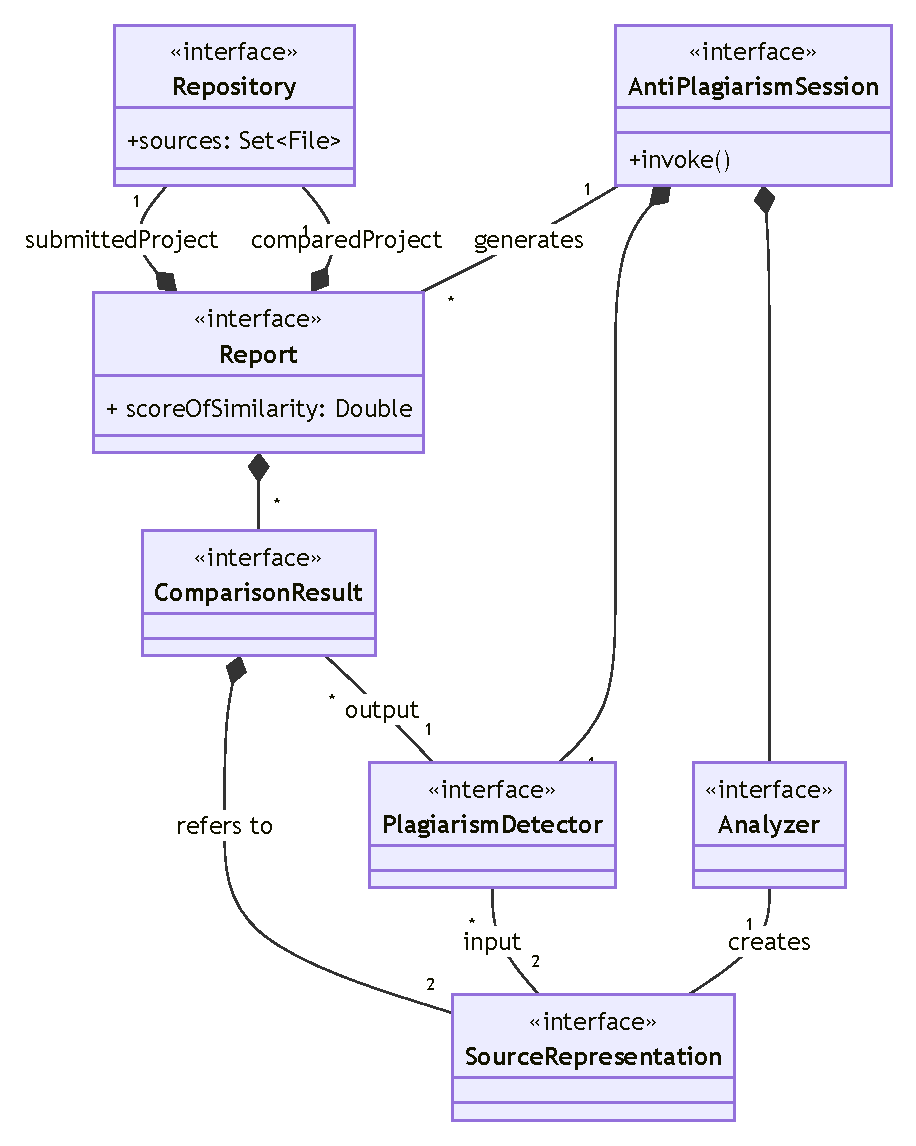
\includegraphics[width=\textwidth]{resources/img/02-domain.pdf}
    \caption{Schema UML delle classi dell'analisi del problema, con rappresentate le entità principali ed i rapporti fra loro.}
    \label{img:02-domain}
\end{figure}

\newpage

\section{\textit{Design}}

\subsection{Architettura}
\label{02-architecture}
L'architettura del sistema è così organizzata: \textbf{\texttt{AntiPlagiarismSession}} è l'interfaccia responsabile della logica dell'applicazione e rappresenta una specifica sessione, dove per sessione si intende l'entità che, una volta opportunamente configurata, esegue la logica dell'applicazione.
%
La configurazione su cui essa opera è reificata nell'interfaccia \texttt{RunConfiguration} e rappresenta un "contenitore" d'informazioni necessarie per l'esecuzione del sistema, tra cui la triade composta da \texttt{Analyzer}, \texttt{Detector} e \texttt{Filter}, nonché le \texttt{Repository} su cui deve essere effettuata l'analisi, a loro volta recuperate da un \texttt{RepositoryProvider} che si occuperà di scaricare i progetti dai servizi di \textit{hosting} che verranno supportati dal sistema.
%
Tale configurazione è creata da un \texttt{RunConfigurator}, a cui spetta la corretta istanziazione in accordo con le opzioni definite dall'utente.

Gli \texttt{Output} rappresentano le risorse su cui \textit{loggare} le informazioni durante l'esecuzione.
%
Un particolare tipo di \texttt{Output} è rappresentato dal \texttt{ReportsExporter}, il componente che si occuperà di esportare opportunamente i risultati dell'analisi.

Infine, \texttt{KnoledgeBaseRepository} rappresenta l'interfaccia che permette il salvataggio e il recupero delle rappresentazioni dei sorgenti già precedentemente analizzate e, perciò, salvate.
%
La tecnica con cui questo verrà realizzato, salvataggio su \textit{file} piuttosto che l'uso di un \textit{database}, è un aspetto tecnologico implementativo che non deve impattare sull'architettura e di cui non si tiene qui conto.

Questa architettura permette di configurare opportunamente ogni sessione in base alle proprie esigenze utilizzando le tecniche e le metriche che si ritengono più consone in relazione al contesto in cui lo strumento viene calato.
%
Inoltre, si lascia aperta la possibilità di estendere le strategie per l'esportazione dei risultati (più in generale dell'\texttt{Output}) e per la creazione della configurazione, nel caso in futuro si voglia aggiungere un'interfaccia grafica al sistema.

In \Cref{img:02-architecture} è esemplificato il diagramma UML architetturale.

\begin{figure}[h!]
    \makebox[\textwidth][c]{
        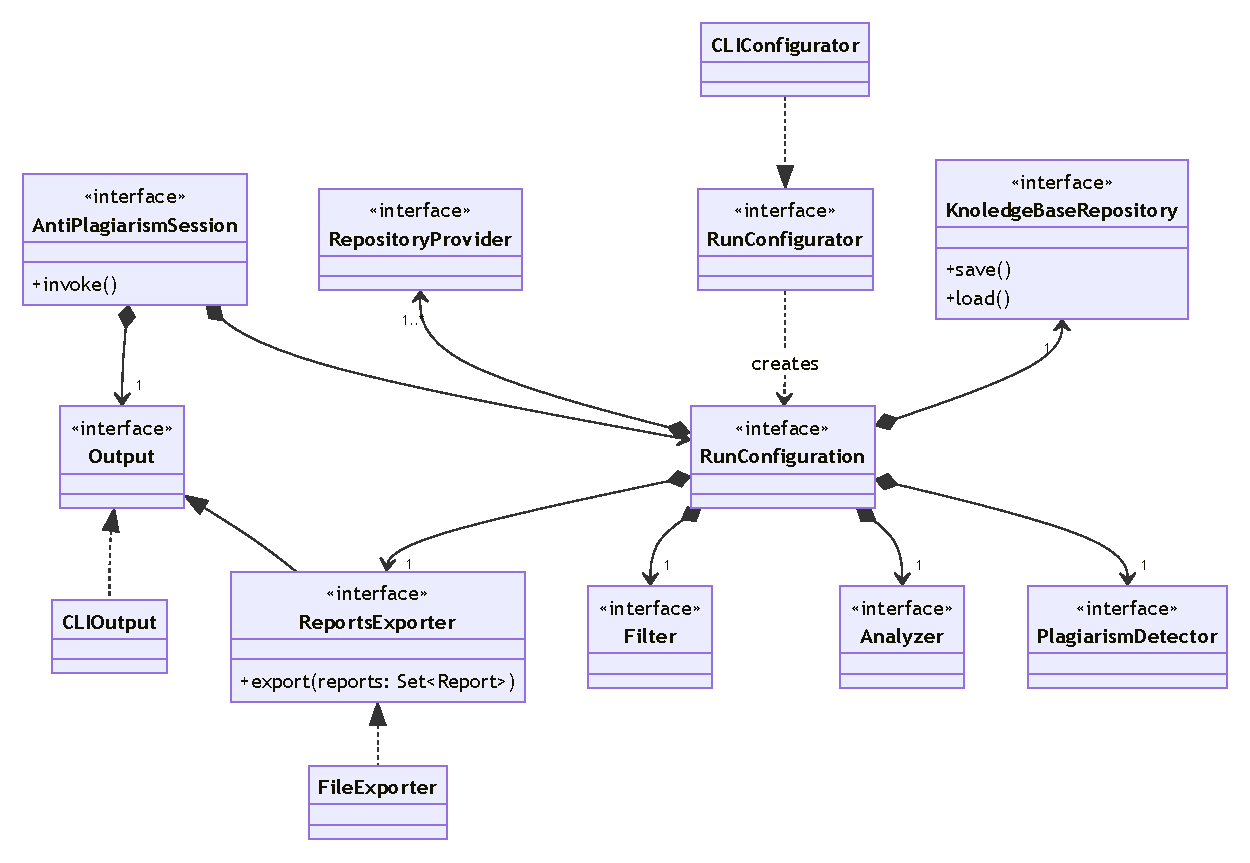
\includegraphics[width=1.1\textwidth]{resources/img/02-achitecture.pdf}
    }
    \caption{Schema UML architetturale del sistema.}
    \label{img:02-architecture}
\end{figure}

\subsection{\textit{Design} dettagliato}

\subsubsection*{\textit{Provider} dei progetti}
Per quanto concerne i \textit{provider} di \textit{repository}, ovvero i componenti che devono recuperare i sorgenti dei progetti da \textit{repository} pubbliche da \textit{GitHub} e/o da \textit{Bitbucket}, si è scelto un \textit{design} che permettesse il massimo riuso degli elementi comuni, aderendo a uno schema interfaccia $-$ classe astratta $-$ classe concreta (\Cref{img:02-provider}).

\begin{figure}[h!]
    \centering
    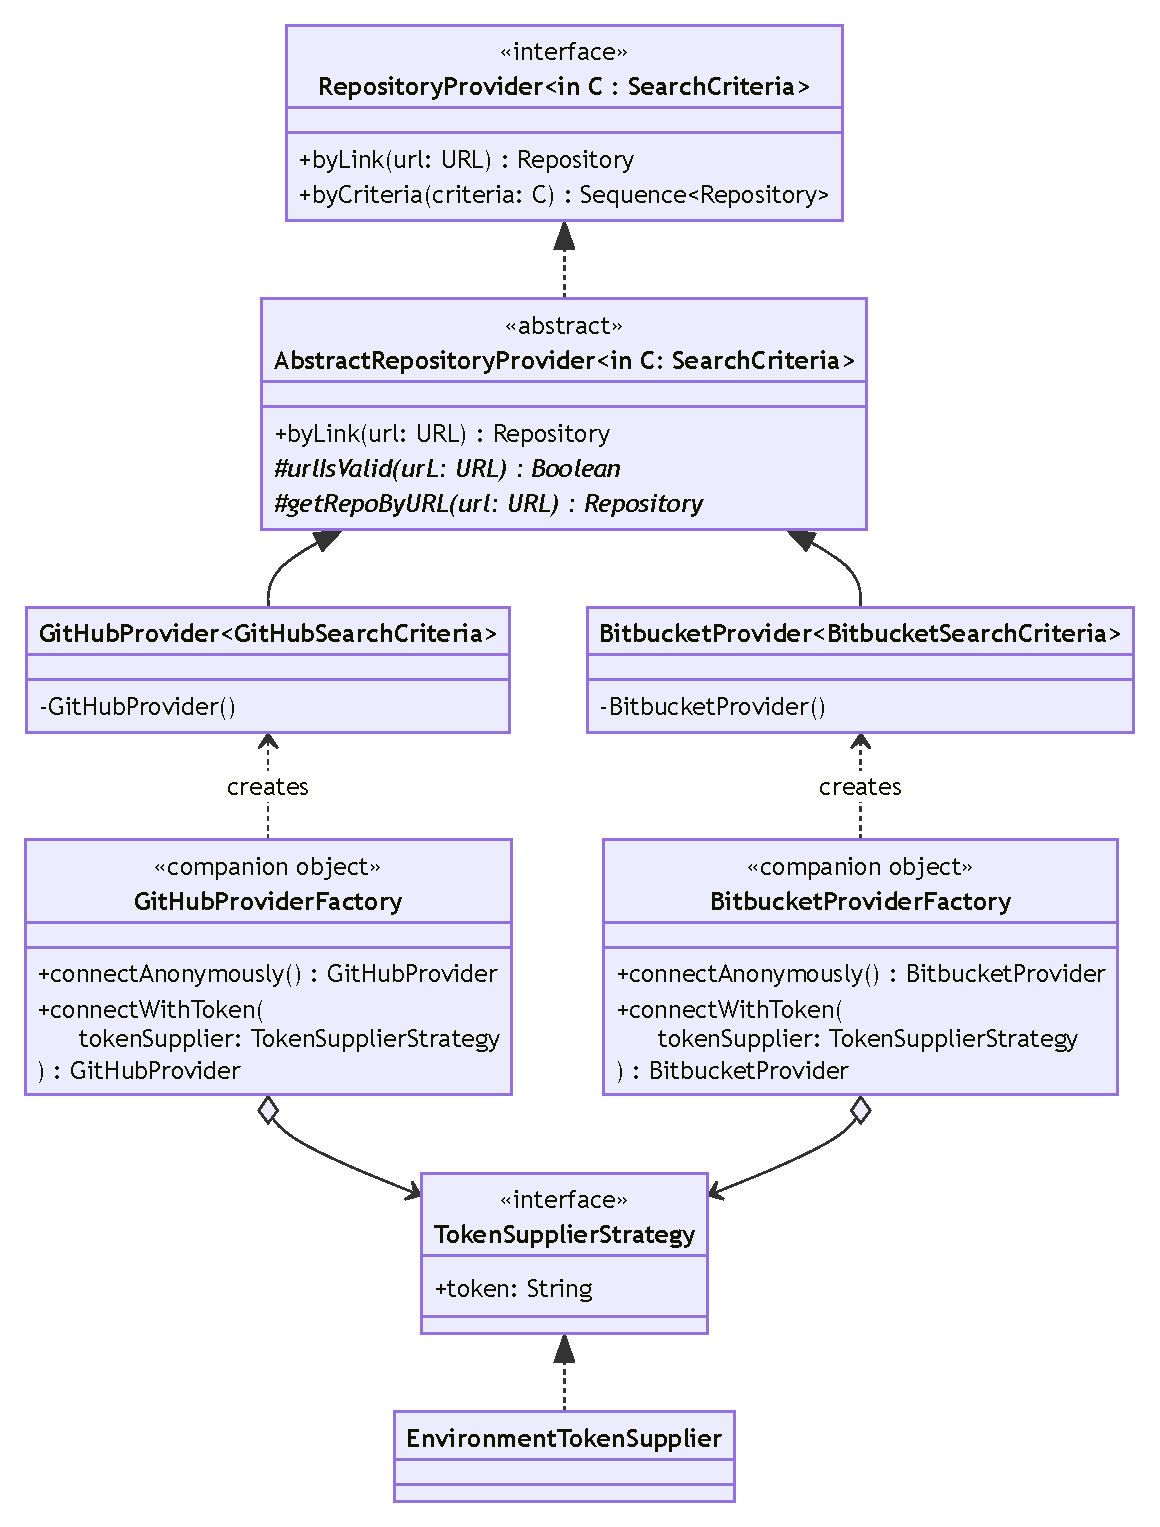
\includegraphics[width=0.9\textwidth]{resources/img/02-provider.pdf}
    \caption{Schema UML dei provider.}
    \label{img:02-provider}
\end{figure}

Viste le limitazioni in termini di numero di richieste che i due servizi impongono\footnote{Sia \textit{GitHub} che \textit{Bitbuckt} hanno un limite massimo di richieste che possono essere effettuate in un certo intervallo di tempo che varia in base la richiesta sia autenticata o meno. Questi vincoli sono imposti per garantire la protezione da attacchi di tipo \textit{Denial of Service}, consentire la scalabilità e garantire buone prestazioni in termini di tempo di risposta.} e la conseguente necessità di autenticarsi mediante degli opportuni \textit{token} per effettuare le richieste \textit{REST}, si è optato di demandare la logica di recupero dei suddetti \textit{token} di autenticazione all'interfaccia \texttt{TokenSupplierStrategy} che reifica il \textit{pattern} \textit{Strategy} \cite{gof}.
%
L'implementazione di \textit{default} ricerca tra variabili d'ambiente, ma altri approcci possono essere introdotti in modo del tutto trasparente ai \textit{provider}.

La creazione dei \textit{provider} avviene per mezzo di due \textit{static factory} \cite{effective-java}, incapsulate all'interno dei due \textit{provider}, in modo da permettere di ottenere un oggetto \textit{provider} anche senza autenticazione.
%
Nonostante questo sia in genere sconsigliato per via delle limitazioni sopra citate, può essere utile in fase di \textit{testing} per permettere di testare il sistema anche in contesti in cui non sia possibile usare \textit{token} di autenticazione validi, ad esempio nel contesto delle \textit{GitHub Actions} nei \textit{workflow} scatenati da eventi di tipo \textit{Pull Request} (si veda \Cref{03-git-ci})

Dopo una prima analisi delle \textit{API} dei due servizi di \textit{hosting} si è convenuto di permettere di recuperare i progetti mediante due metodi: un \textit{link} diretto alla \textit{repository}, oppure mediante un criterio di ricerca, rappresentato dall'interfaccia \texttt{SearchCriteria}.
%
Per permettere che questi siano componibili è stato qui utilizzato il pattern \textit{Decorator} \cite{gof}.
%
La classe astratta che funge da decoratore è \texttt{(GitHub|BitBucket)CompoundCriteria} e le sue concrete implementazioni permettono di specificare il nome della \textit{repository} o il linguaggio.
%
In questo modo possono essere creati dinamicamente criteri compositi in base alle esigenze del \textit{client} e in futuro potrebbero essere aggiunti nuovi criteri di ricerca, come, ad esempio, il numero di stelle ricevute o la data di creazione, aderendo all'\textit{Open Closed Principle} secondo cui le entità di un sistema devono essere aperte all'estensione, ma chiuse alla modifica.
%
Il \textit{design} è presentato in \Cref{img:02-search-criteria}.

\begin{sidewaysfigure}
    \centering
    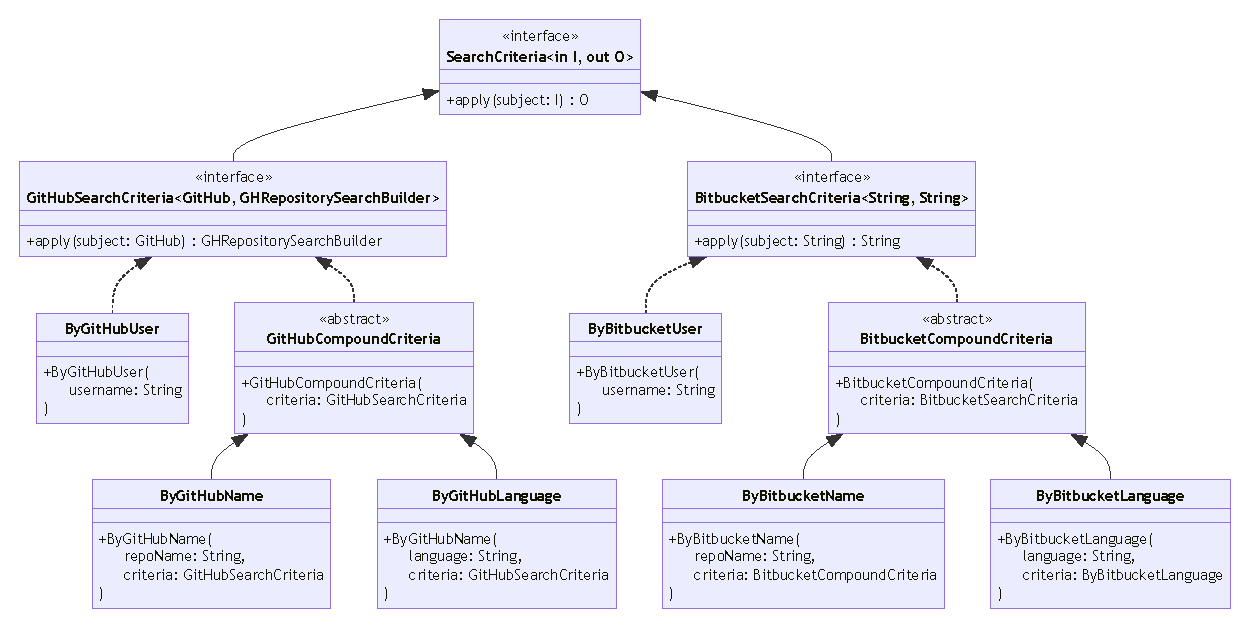
\includegraphics[width=\textwidth]{resources/img/02-search-criteria.pdf}
    \caption{Schema UML dei criteri di ricerca delle \textit{repository}.}
    \label{img:02-search-criteria}
\end{sidewaysfigure}

Le \textit{repository} sono modellate attraverso l'omonima interfaccia, le cui concrete implementazioni rappresentano degli \textit{Adapter} \cite{gof} alle interfacce di libreria utilizzate (si veda \Cref{img:02-repos}).
%
Questo permette di essere indipendenti dalla specifica libreria utilizzata, che rimane un dettaglio implementativo, e avere un livello di astrazione adeguato al contesto applicativo.

Per quanto attiene il salvataggio dei sorgenti e il loro recupero, in modo tale che possano essere riusati in sessioni successive senza dover essere ri-scaricati, è affidato ad un gestore rappresentato dall'interfaccia \texttt{KnoledgeBaseManager}.
%
Per il momento, la tecnica utilizzata consiste nel salvare i sorgenti in locale.
%
Per tale motivo, la concreta implementazione \texttt{FileKnowledgeBaseManager} si occupa di scaricare i progetti, "ripulirli" da artefatti non importanti ai fini dell'analisi, come i file di configurazione di Gradle, e infine salvarli in un'apposita cartella di sistema.
%
Nel momento in cui è necessario recuperare i sorgenti di un progetto ci si interfaccia con il gestore chiedendogli di fornire tutti i sorgenti disponibili per quel determinato progetto, già precedentemente salvati.

Un indomani, se si volesse sostituire questo metodo di \textit{caching} con uno più avanzato, di cui oggi non se ne ravvisa l'esigenza, si potrebbe implementare un nuovo \texttt{KnoledgeBaseManager}.

\begin{figure}[h!]
    \makebox[\textwidth][c]{
        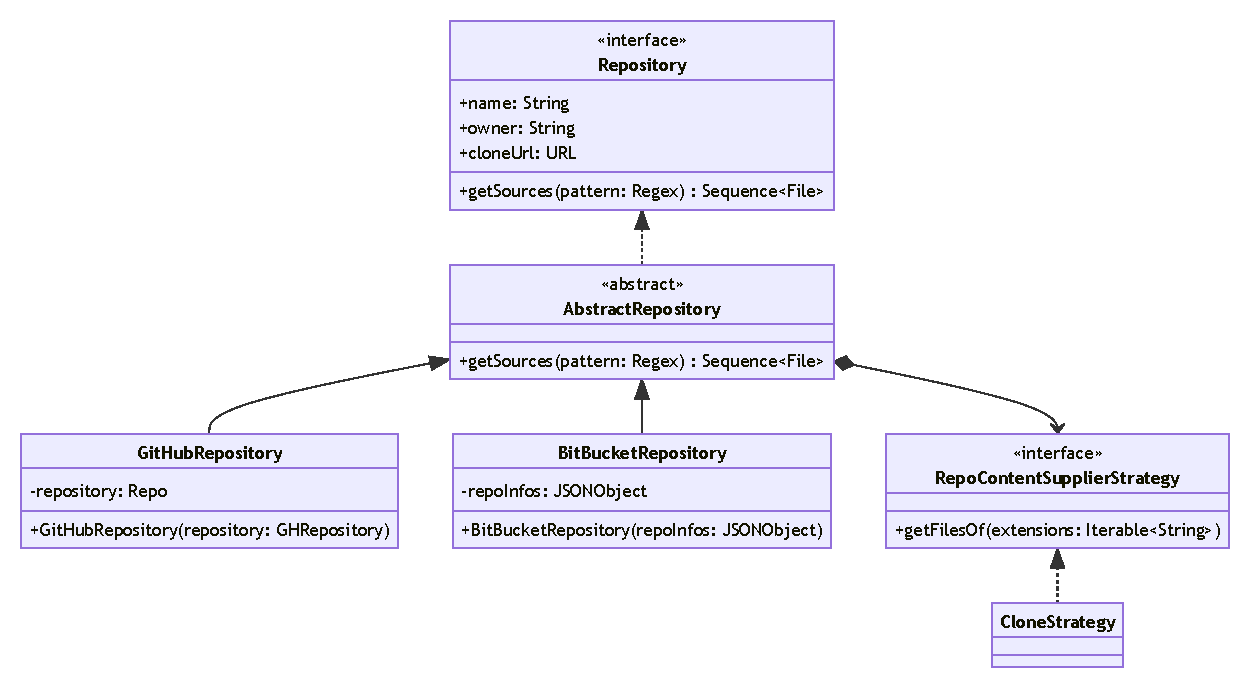
\includegraphics[width=1.15\textwidth]{resources/img/02-repos.pdf}
        }
    \caption{Schema UML delle \textit{repository} e del gestore dei loro sorgenti.}
    \label{img:02-repos}
\end{figure}

\subsubsection*{Analizzatore e \textit{detector}}
L'analizzatore, il \textit{filter} e il \textit{detector} sono il cuore dell'intero sistema.
%
Il loro \textit{design} è stato pensato in modo tale da permettere il massimo grado di configurabilità e di estendibilità.
%
Presumibilmente, infatti, questi sono i componenti che varieranno più spesso nell'arco del ciclo di vita di questo \textit{software} e il cui grado di configurabilità influirà certamentente in modo preponderante sia sulle prestazioni, sia sull'efficacia del sistema.

Tutti e tre i componenti sono stati progettati, in stile funzionale, come delle funzioni che, preso in \textit{input} uno più argomenti, ritornano in \textit{output} l'\textit{input} del componente successivo.
%
L'esecuzione di una tecnica è, infatti, una catena di funzioni applicate in sequenza.

L'analizzatore è il componente che si occupa di trasformare i file sorgenti in rappresentazioni confrontabili.
%
Indipendentemente dalla tipologia di analisi che si voglia applicare, la trasformazione non avviene tramite un semplice passaggio, bensì una sequenza di operazioni che sono eseguite sequenzialmente in cascata.
%
Nel caso in esame, queste sono: il \textit{parsing} del file, una fase di \textit{preprocessing} ed infine la \textit{tokenizzazione} del sorgente.
%
Questa sequenza di azioni è naturalmente modellata attraverso il pattern \textit{Pipeline} \cite{pipeline-pattern}: ogni singolo stadio è modellato attraverso l'interfaccia \texttt{StepHandler} e la \textit{pipeline} viene costruita all'interno del concreto \texttt{Analyzer}, nel nostro caso \texttt{JavaTokenizationAnalyzer}.
%
Il \textit{design} dell'analizzatore è esemplificato in \Cref{img:02-analyzer}.

\begin{figure}[h!]
    \makebox[\textwidth][c]{
        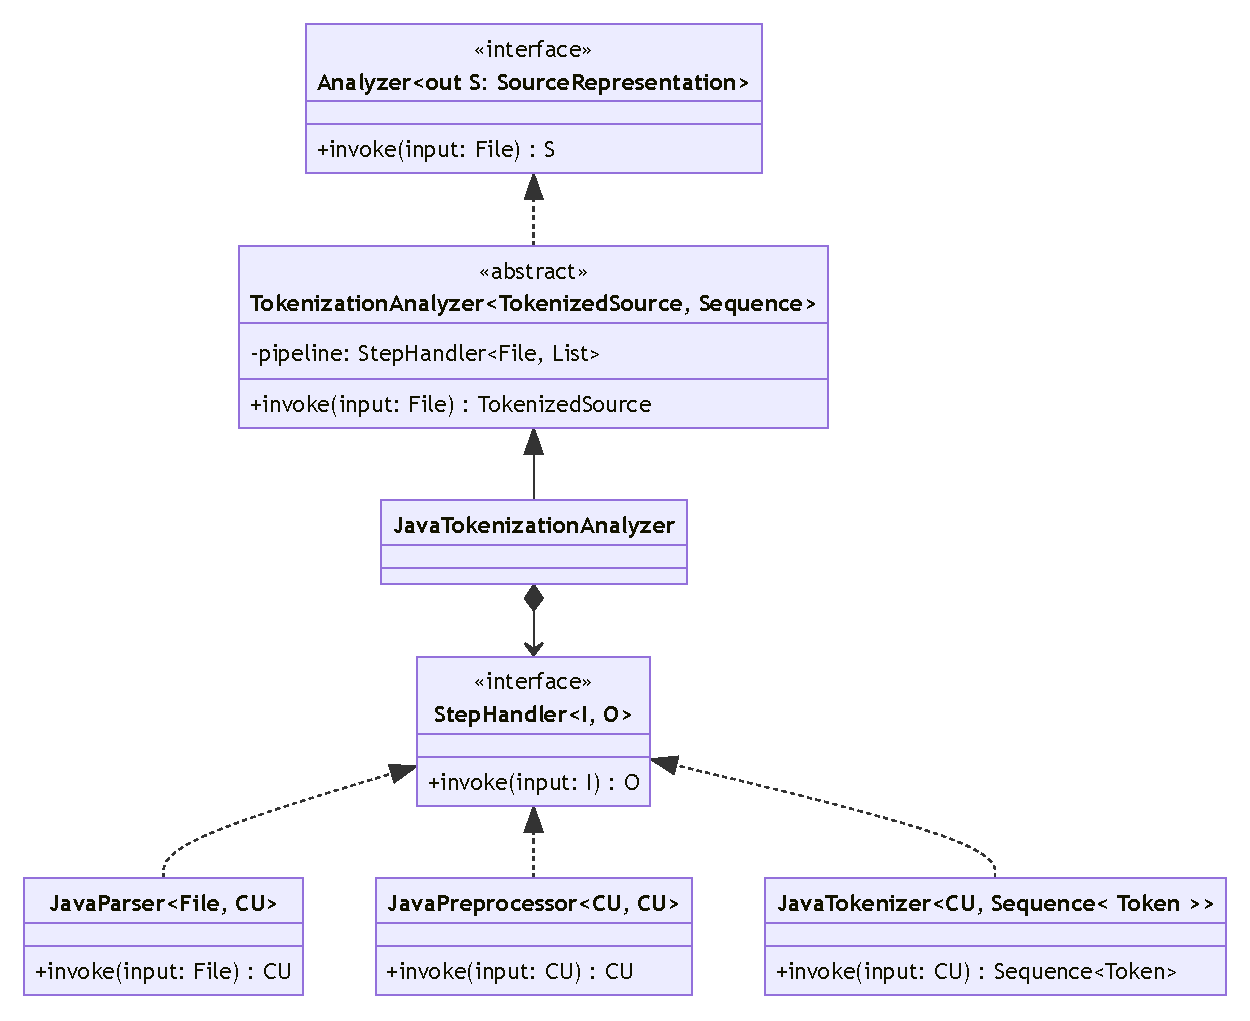
\includegraphics[width=1.12\textwidth]{resources/img/02-analyzer.pdf}
    }
    \caption{Schema UML dell'analizzatore.}
    \label{img:02-analyzer}
\end{figure}

La rappresentazione intermedia prodotta dall'analizzatore è modellata dall'interfaccia \texttt{SourceRepresentation} (\Cref{img:02-representations}). 
%
Tra tutte, quella implementata nell'attuale sistema è composta da una sequenza di \textit{token} e perciò denominata \texttt{TokenizedSource}.
%
L'elenco dei possibili tipi di \textit{token} che la compongono dipende chiaramente dal linguaggio utilizzato.
%
La strategia di recupero di questi ultimi è affidata, al solito tramite \textit{Strategy}, all'interfaccia \texttt{TokenTypesSupplier}, la cui implementazione di \textit{default} effettua la de-serializzazione di un file di configurazione in cui sono salvate tutte le tipologie di \textit{token}.

\begin{figure}[h!]
    \centering
    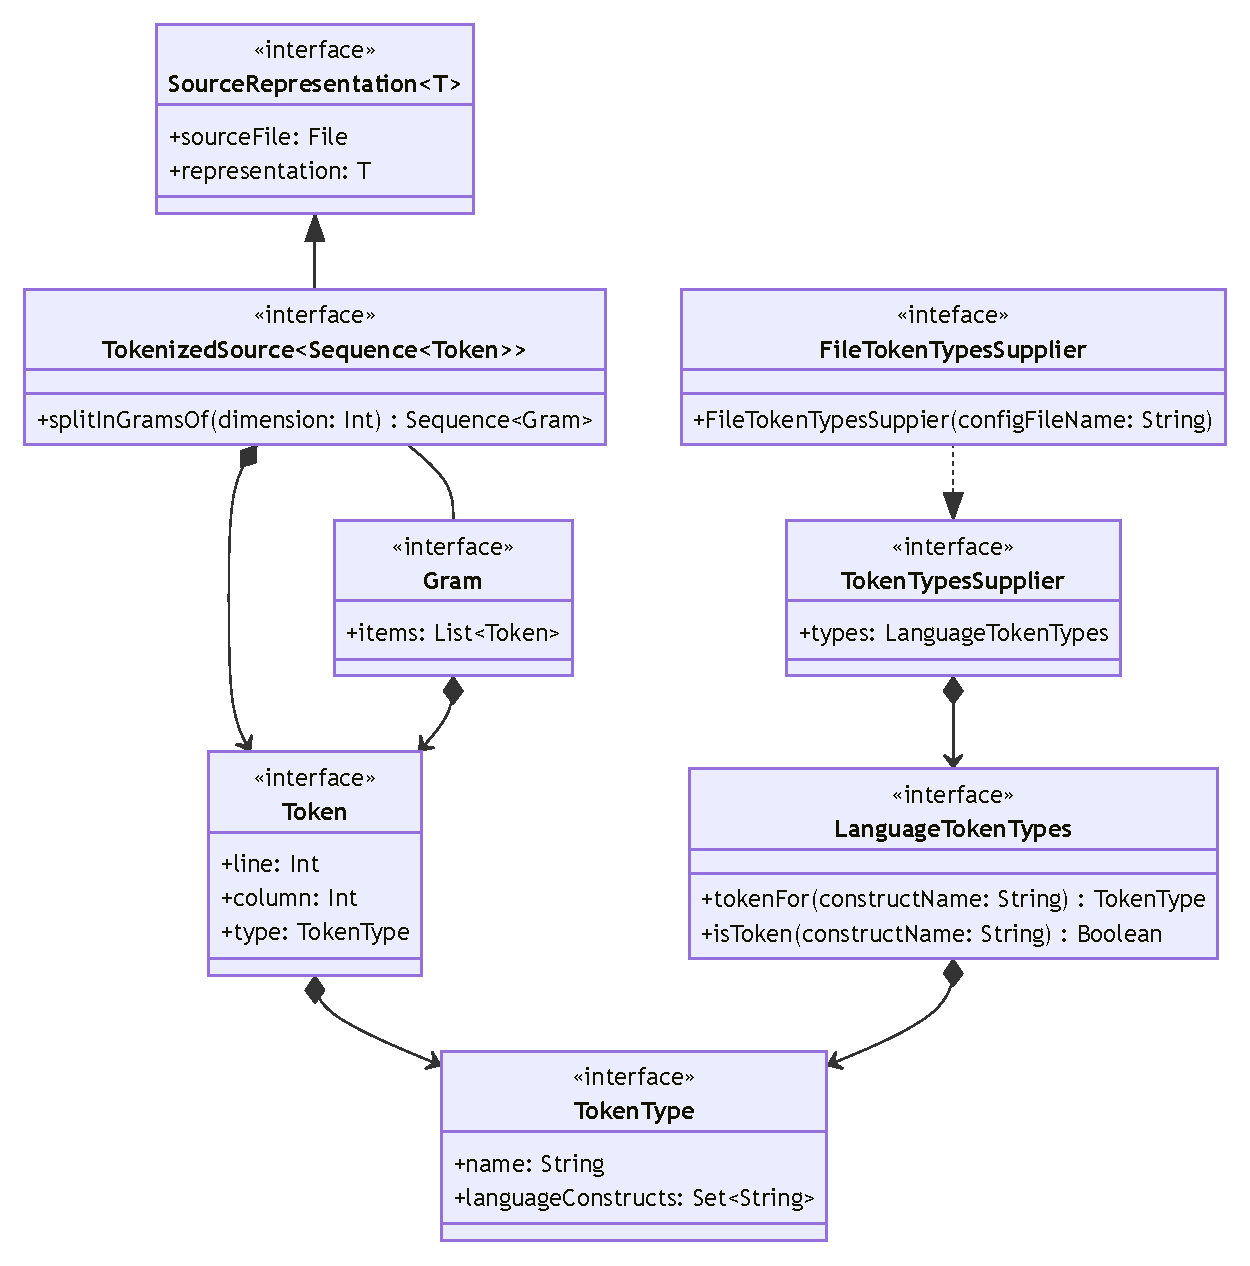
\includegraphics[width=\textwidth]{resources/img/02-representations.pdf}
    \caption{Schema UML delle rappresentazioni intermedie.}
    \label{img:02-representations}
\end{figure}

Le rappresentazioni generate dal processo di analisi, vengono poi opportunamente filtrate per mezzo di un \texttt{RepresentationFilter} che, preso in \textit{input} una istanza dell'insieme delle \textit{submission} e l'insieme del \textit{corpus} con cui confrontarla, ne effettua un filtraggio secondo opportune metriche.
%
Per farlo, fa uso di un \texttt{Indexer} che crea, a partire dalle rappresentazioni, indici (strutture dati) su cui poter calcolare stime di similarità.
%
Uno schema di massima è presentato in \Cref{img:02-filter}

\begin{figure}[h!]
    \centering
    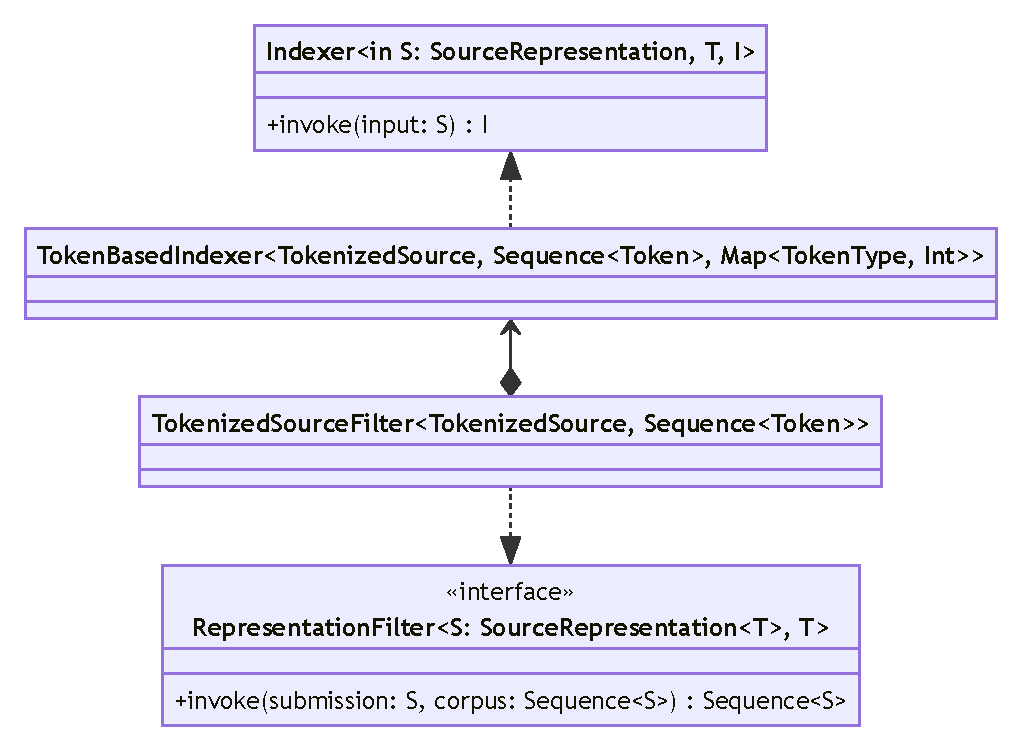
\includegraphics[width=0.9\textwidth]{resources/img/02-filter.pdf}
    \caption{Schema UML del filtro.}
    \label{img:02-filter}
\end{figure}

\texttt{PlagiarismDetector} (\Cref{img:02-detector}) rappresenta invece il componente che individua le similarità tra una coppia di \texttt{SourceRepresentation} e si occupa di calcolare la loro similarità.
%
Poiché vi sono una molteplicità di algoritmi presenti in letteratura che assolvono a questo compito, si è deciso d'implementarli sotto forma di gerarchia di classi di algoritmi il cui contratto comune è definito da \texttt{ComparisonStrategy}. 
%
In particolare, ogni classe implementante \texttt{ComparisonStrategy} genera un \texttt{Match}, dove per \texttt{Match} si intende due sezioni simili di \texttt{SourceRepresentation}.
%
L'insieme dei \texttt{Match} che compongono la comparazione di due \texttt{SourceRepresentation} sono raggruppate in un \texttt{ComparisonResult}, il cui grado di similarità è stimato dalla \texttt{SimilarityEstimationStrategy}.

Nel contesto della \textit{tokenizzazione}, i due concreti algoritmi che sono implementati come strategia di confronto sono rappresentati dalle sottoclassi \texttt{GreedyStringTiling} e \texttt{RKRGreedyStringTiling}.
%
Entrambi generano dei \texttt{TokenMatch}, costituiti da sequenze contigue di \textit{token} dello stesso tipo.
%
A partire da queste la classe concreta \texttt{TokenBasedPlagiarismDetector} demanda alle concrete implementazioni di \texttt{TokenBasedSimilarityStrategy} il calcolo della similarità.

\begin{sidewaysfigure}
    \makebox[\textwidth][c]{
        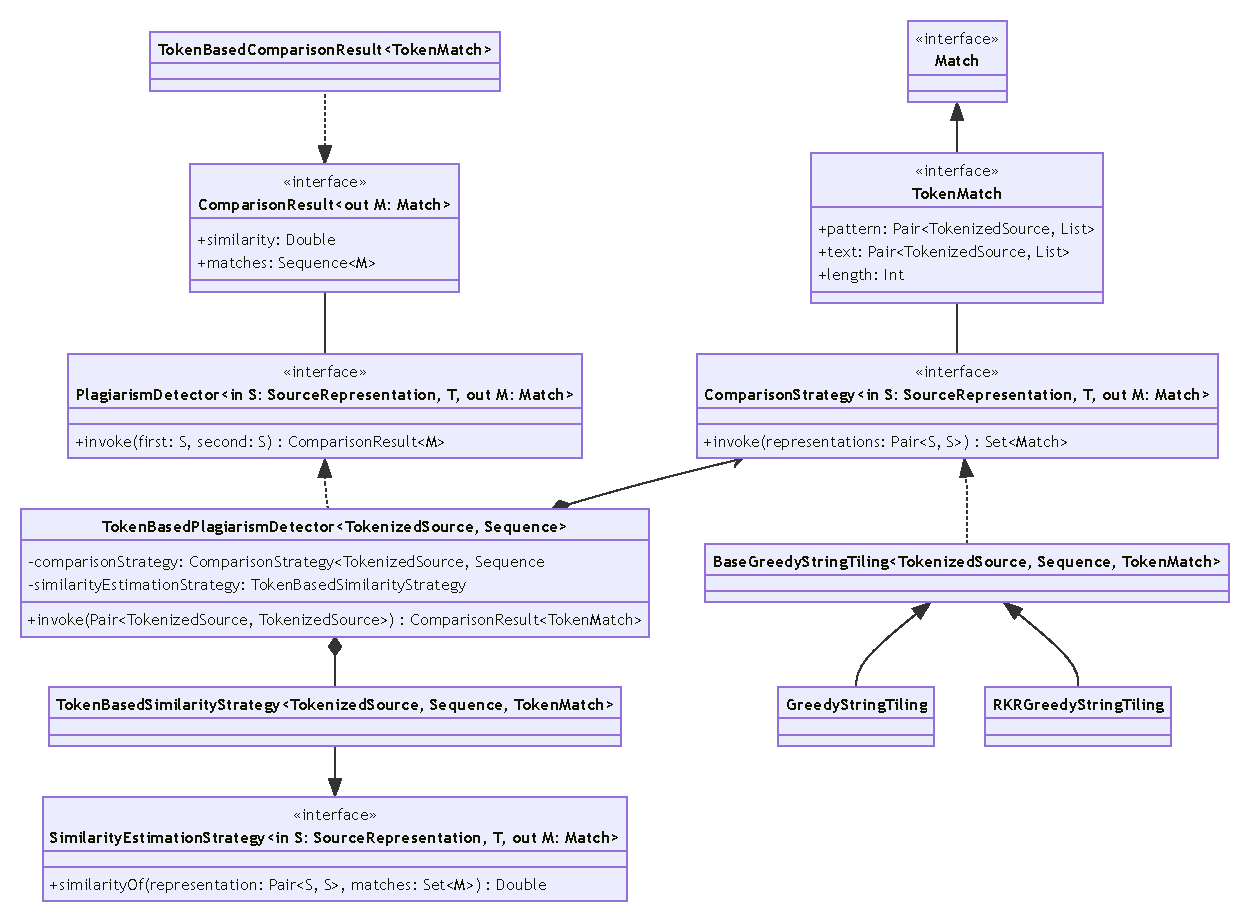
\includegraphics[width=1.22\textwidth]{resources/img/02-detector.pdf}
    }
    \caption{Schema UML del \textit{detector}.}
    \label{img:02-detector}
\end{sidewaysfigure}

\newpage

Tutti e tre i componenti, \texttt{Analyzer}, \texttt{Filter} e \texttt{PlagiarismDetector}, sono incapsulati all'interno di un concreto \texttt{TechniqueFacade} \cite{gof}.
%
Si è deciso di adottare questo approccio principalmente per due motivi:
\begin{itemize}
    \item la specifiche strategie di analisi e di confronto devono essere istanziate e opportunamente configurate a \textit{runtime} a seconda del tipo di tecnica e delle opzioni scelte dall'utente. Inoltre, devono essere coerenti tra loro: non è possibile, ad esempio, poter istanziare un analizzatore per effettuare la \textit{tokenizzazione} e un rilevatore che non operi sulla sequenza di \textit{token}. Il \textit{facade} pertanto si occupa d'istanziare i corretti componenti necessari all'esecuzione della tecnica in accordo con i parametri a lui fornitogli, sollevando il \textit{client} da questa responsabilità.
    \item Il processo di analisi e confronto può essere complesso. Pertanto si fornisce ai \textit{client} un'interfaccia semplificata che assolve al compito di eseguire una generica tecnica, rendendo di fatto trasparente al chiamante la complessità del sottosistema che, dal suo punto di vista, è di fatto una \textit{black box}.
\end{itemize}

\subsubsection*{Configurabilità, Input e Output}

Come già detto, l'aspetto della configurabilità è un aspetto molto importante in questo contesto, in quanto la scelta dei parametri influisce sull'efficacia del rilevamento.
%
Come già presentato nell'architettura, una specifica sessione è legata ad una particolare configurazione (\texttt{RunConfiguration}) che contiene tutte le informazioni necessarie per l'esecuzione della stessa.
%
A differenza di quanto presentato nella \Cref{02-architecture}, giacché per i motivi suddetti \texttt{Analyzer}, \texttt{Filter} e \texttt{Detector} sono stati incapsulati all'interno della \texttt{TechniqueFacade}, la configurazione non ha un riferimento diretto a ciascuno dei tre componenti, bensì all'oggetto \textit{facade}.

L'attuale \texttt{ReportsExporter} implementato esporta i dati in un semplice \textit{file} di testo e i \texttt{RunConfigurator} attualmente supportati sono il \texttt{CLIConfigurator}, che crea la configurazione a partire dagli argomenti da riga di comando, oppure il \texttt{FileConfigurator} che sfrutta un file di configurazione per impostare tutti i parametri.
%
In futuro, il design potrebbe essere esteso per supportare un'interfaccia grafica per la configurazione o per generare \textit{report} più ricchi in termini di presentazione (ad esempio un file \textit{HTML}).

In \Cref{img:02-session} è mostrato lo schema UML delle classi che mostra complessivamente i rapporti tra le varie componenti.

\begin{sidewaysfigure}
    \makebox[\textwidth][c]{
        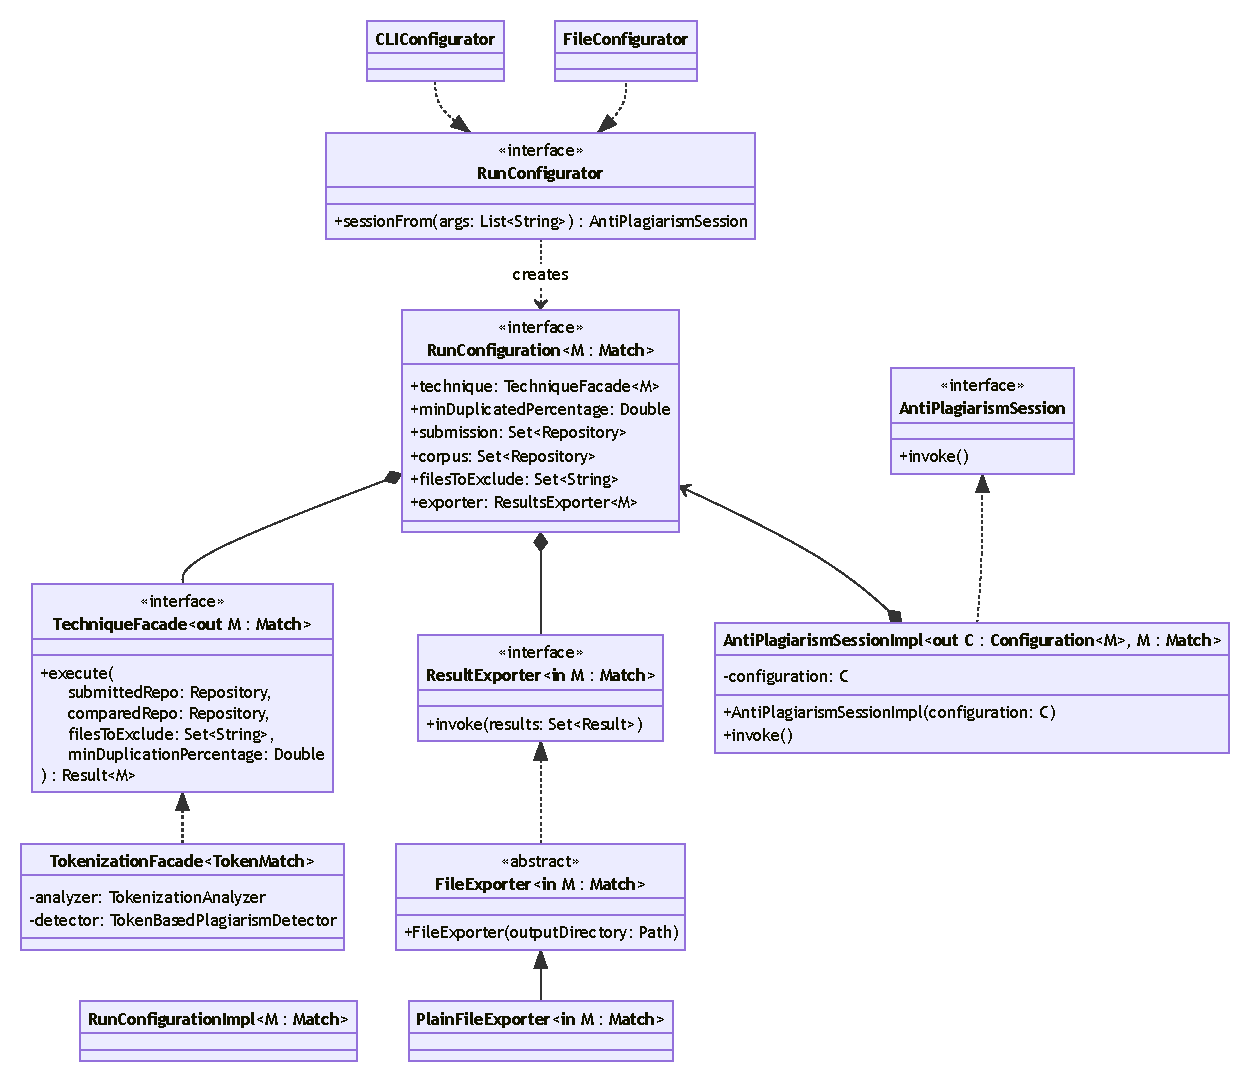
\includegraphics[width=1\textheight]{resources/img/02-session.pdf}
    }
    \caption{Schema UML della sessione}
    \label{img:02-session}
\end{sidewaysfigure}

\subsubsection*{Comportamento}
Per concludere, in \Cref{img:02-sequence-diagram} viene mostrato il diagramma UML di sequenza che mostra macroscopicamente il flusso delle azioni del sistema e come le varie componenti cooperano tra loro.

\begin{figure}[h!]
    \hspace*{-3.4cm}
    \makebox[\textwidth][l]{
        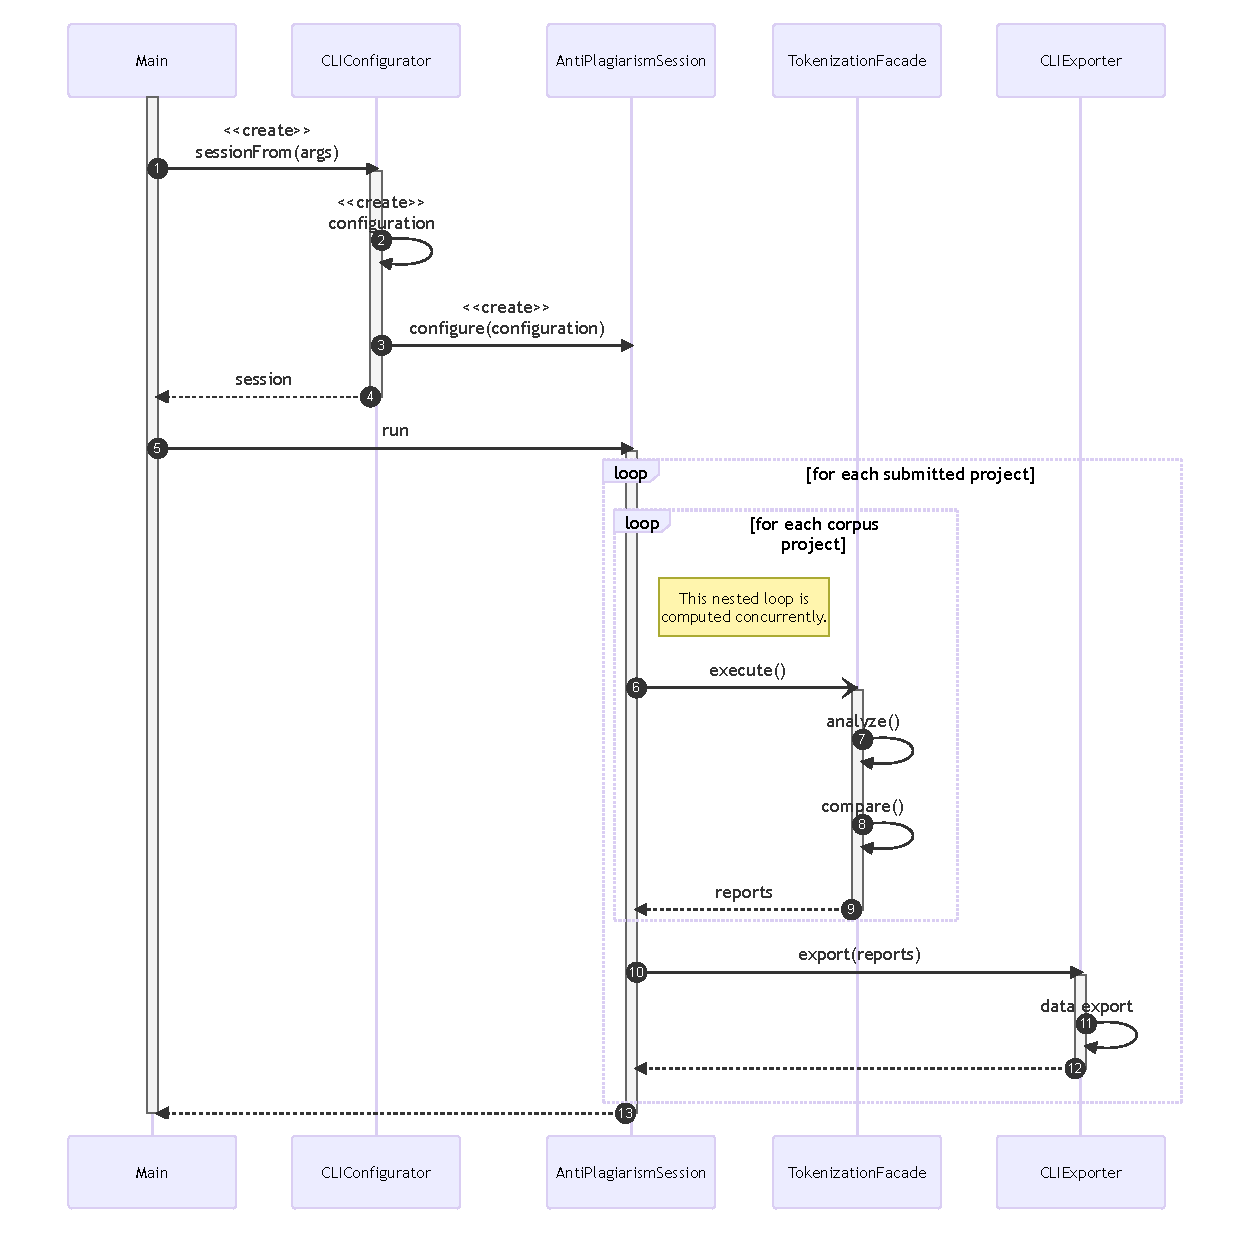
\includegraphics[width=1.35\textwidth]{resources/img/02-sequence-diagram.pdf}
    }
    \hspace*{1cm}
    \caption{Diagramma UML di sequenza rappresentante l'interazione tra le componenti del sistema.}
    \label{img:02-sequence-diagram}
\end{figure}
